%%%%%%%% NeurIPS 2025 STYLE %%%%%%%%%%%%%%%%%

\documentclass{article}

\usepackage[preprint]{neurips_2025}

\usepackage[utf8]{inputenc}
\usepackage[T1]{fontenc}
\usepackage{hyperref}
\usepackage{url}
\usepackage{booktabs}
\usepackage{amsfonts}
\usepackage{nicefrac}
\usepackage{microtype}

% Recommended, but optional, packages for figures and better typesetting:
\usepackage{graphicx}
\usepackage{subcaption}

% Attempt to make hyperref and algorithmic work together better:
\newcommand{\theHalgorithm}{\arabic{algorithm}}

\usepackage{amsmath}
\usepackage{amssymb}
\usepackage{mathtools}
\usepackage{amsthm}
\usepackage[capitalize,noabbrev]{cleveref}
\usepackage{xcolor}
\usepackage{multirow}
\usepackage{balance}

% Avoid stretched vertical whitespace in two-column layout.
\raggedbottom

\title{The Shape of Wisdom}
\author{%
  \textbf{Shailesh Rana} \\
  Independent Researcher \\
  \And
  \textbf{Claude Opus 4.6} \\
  \And
  \textbf{ChatGPT Prism} \\
}

\makeatletter
\renewcommand{\@notice}{}
\makeatother

\begin{document}

\twocolumn[
\begin{@twocolumnfalse}
\maketitle

%% ============================================================
%% ABSTRACT
%% ============================================================
\begin{abstract}
We introduce three quantities---\emph{state}, \emph{motion}, and \emph{boundary}---that fully describe the layer-by-layer trajectory of a transformer's answer on multiple-choice benchmarks.
The \textbf{state} is the logit margin between the model's preferred answer and its strongest competitor at each layer.
\textbf{Motion} is the per-layer change in that margin.
\textbf{Boundary} is its absolute magnitude, measuring proximity to a decision flip.
Across three 7--8B instruction-tuned transformers, these primitives separate prompts into four trajectory types---\emph{stable-correct}, \emph{stable-wrong}, \emph{unstable-correct}, and \emph{unstable-wrong}---producing a phase diagram that replicates across models and knowledge domains.
We decompose motion into attention-driven \emph{routing} and MLP-driven \emph{injection}, achieving reconstruction $R^2 \geq 0.70$ on held-out data.
Linearized counterfactual accounting via simulated component removal, activation substitution, and input-level span-deletion experiments---controlled against shuffled and sign-flipped baselines with Benjamini--Hochberg correction---confirms directionally consistent, finite effects on the decision margin.
\end{abstract}
\vspace{0.2cm}
\end{@twocolumnfalse}
]

%% ============================================================
%% 1. INTRODUCTION
%% ============================================================
\section{Introduction}

A transformer answering a multiple-choice question does not make a single decision.  It makes one decision per layer.  At layer zero the output logits are largely uninformed; by the final layer they commit to an answer.  What happens in between---whether the trajectory converges smoothly, oscillates, or drifts into the wrong basin---determines whether the model answers correctly.

Prior work in mechanistic interpretability has illuminated transformer internals through probing classifiers~\cite{belinkov2022}, causal tracing~\cite{meng2022}, and circuit-level analysis~\cite{olsson2022,conmy2023}.
These approaches identify \emph{what} a model knows and \emph{where} it stores that knowledge, yet typically treat the final output as a binary event rather than examining the dynamic \emph{process} by which the model arrives at it across its full depth.

We propose a complementary perspective.  Rather than asking what a model has learned, we ask: \emph{what does the trajectory of a model's decision look like as it propagates through layers, and can we predict convergence outcomes from a small set of trajectory-level quantities?}

Our answer is yes.  We define three primitives---\textbf{state} (the logit margin~$\delta$), \textbf{motion} (per-layer drift~$g$), and \textbf{boundary} (the absolute margin~$|\delta|$)---and show that they suffice to classify decision trajectories into four outcome types that replicate across models and domains.  We then decompose motion into attention and MLP contributions and assess the resulting mechanistic claims via counterfactual accounting.

\paragraph{Contributions.}
\begin{enumerate}
\item A physics-inspired framework for analyzing transformer decisions as trajectories in logit-margin space, characterized by three measurable quantities.
\item A phase diagram with four well-separated trajectory types, replicated across three architectures and multiple knowledge domains.
\item A linear decomposition of per-layer drift into attention and MLP components with $R^2 \geq 0.70$ on held-out data and a mechanistic interpretation of routing versus injection.
\item Counterfactual accounting experiments---simulated component removal, activation substitution, and input-level span deletion---with multiple-comparison-corrected tests and negative controls.
\end{enumerate}


%% ============================================================
%% 2. THE THREE PRIMITIVES
%% ============================================================
\section{Margin, Drift, and Boundary}
\label{sec:primitives}

We study four-choice (A/B/C/D) questions.  At each transformer layer $l \in \{0,\ldots,L{-}1\}$, we extract logits for the four answer tokens and define all quantities in the restricted four-candidate subspace.  All logits, probabilities, and correctness decisions reported in this paper are computed over the set $\{\mathrm{A}, \mathrm{B}, \mathrm{C}, \mathrm{D}\}$ only; this is a \emph{restricted-choice} readout, not a full-vocabulary prediction.  Correctness is determined by argmax within these four tokens at the final transformer layer.

\subsection{State: The Decision Margin}

Let $z_c(l)$ denote the logit for the correct answer and $z_{k^*}(l)$ the logit for the strongest competitor---the highest-scoring incorrect option.  The \textbf{decision margin} is:
\begin{equation}
  \delta(l) = z_c(l) - z_{k^*}(l).
  \label{eq:delta}
\end{equation}
When $\delta(l) > 0$ the model favors the correct answer; the sign at the final layer determines correctness.

\emph{Design decision.}  We track competitor identity $k^*(l)$ per layer rather than fixing it globally.  A sign flip in $\delta$ can arise from evidence reversal or competitor switch; we report both.

\subsection{Motion: Layer-by-Layer Drift}

The \textbf{drift} is the per-layer change in decision margin:
\begin{equation}
  g(l) = \delta(l{+}1) - \delta(l),
  \label{eq:drift}
\end{equation}
with $g(L) \equiv 0$.  Positive drift moves toward the correct answer.

\subsection{Boundary Proximity}

The \textbf{boundary distance} is the unsigned state:
\begin{equation}
  b(l) = |\delta(l)|.
  \label{eq:boundary}
\end{equation}
Small $b$ means proximity to a decision flip.

\subsection{Convergence and Trajectory Types}

A trajectory is \textbf{stable} if, within a tail window of the last $\tau$ layers, $\delta(l)$ maintains a consistent sign and $b(l) \geq b_{\min}$ throughout.  Combined with final-layer correctness this yields four types: \emph{stable-correct}, \emph{stable-wrong}, \emph{unstable-correct}, \emph{unstable-wrong}.

We use $\tau = 8$, require zero sign flips, and enforce $b_{\min} = 0.3$.  These thresholds were pre-registered.  Sensitivity analysis appears in \cref{sec:appendix_sensitivity}.


\begin{figure*}[t]
  \vskip 0.1in
  \begin{center}
    \centerline{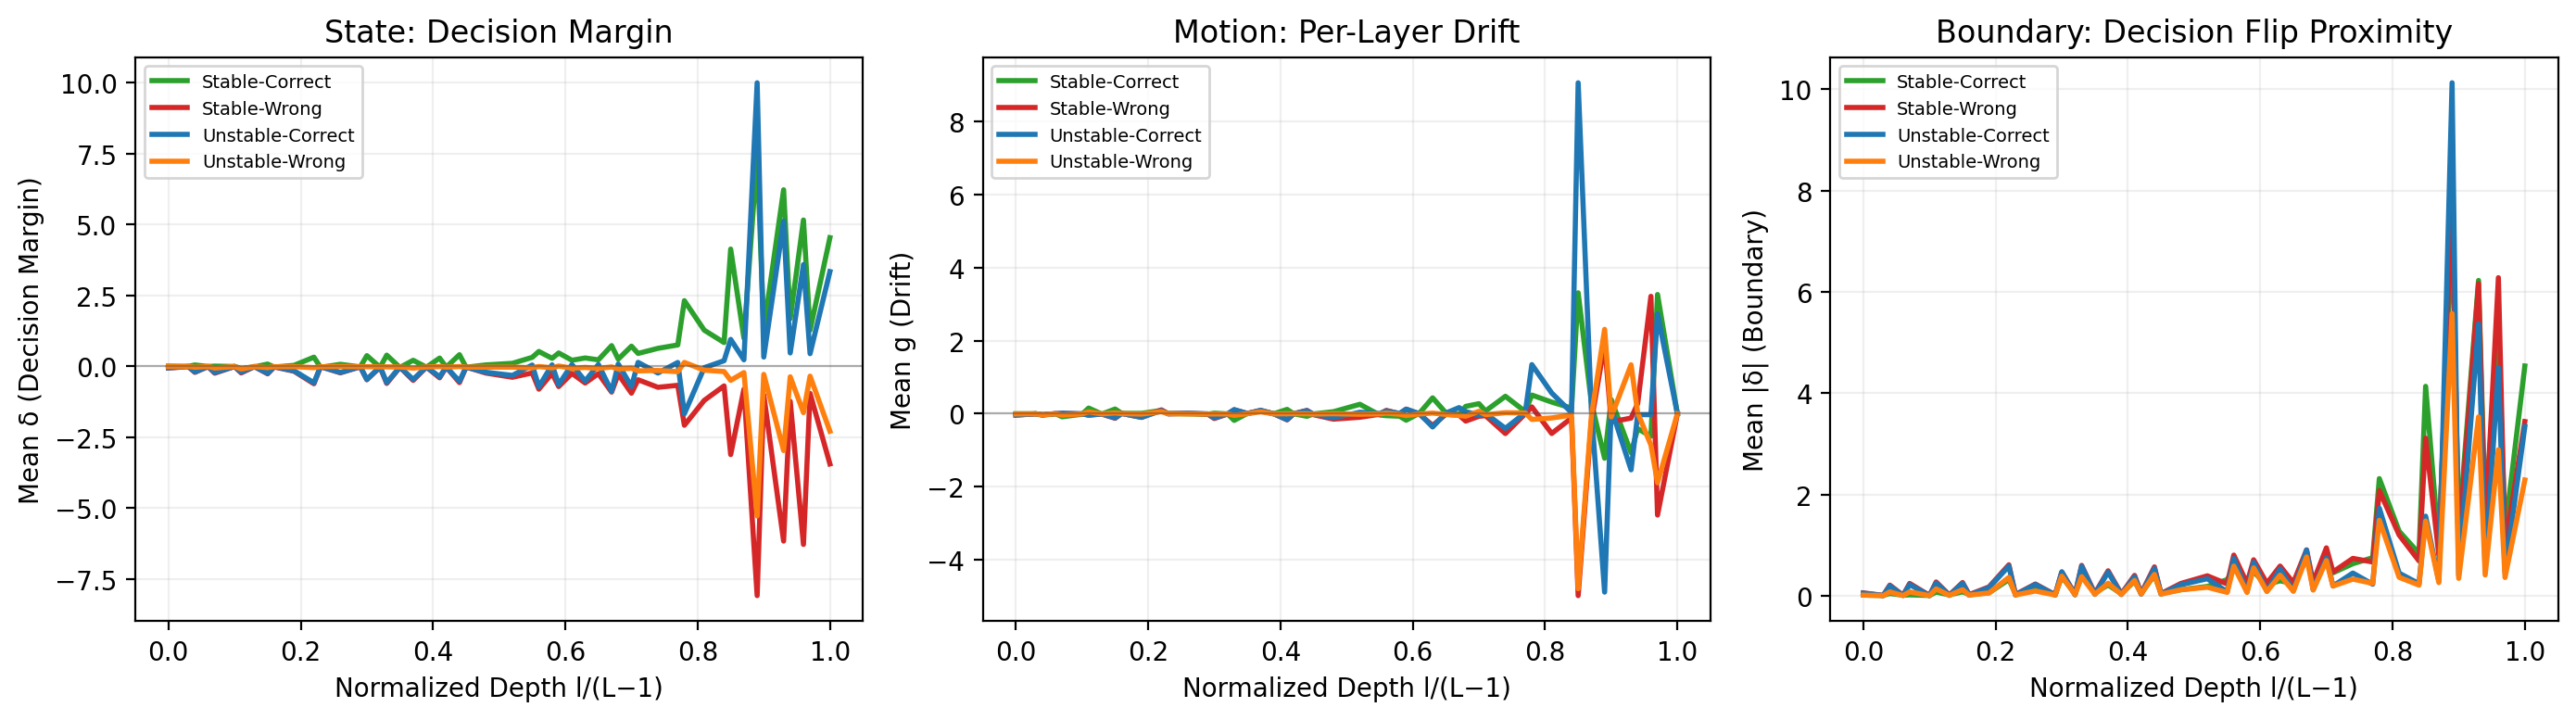
\includegraphics[width=0.95\textwidth]{fig1_three_primitives.png}}
    \caption{The three primitives and four trajectory types, averaged across all three models with layer depth normalized to $[0,1]$.  \textbf{Left:}~Mean decision margin $\delta$ by trajectory type.  \textbf{Center:}~Mean per-layer drift $g$.  \textbf{Right:}~Mean boundary distance $|\delta|$.}
    \label{fig:primitives}
  \end{center}
\end{figure*}


%% ============================================================
%% 3. EXPERIMENTAL SETTING
%% ============================================================
\section{Experimental Setup}
\label{sec:experiments}

\subsection{Models}

We study three instruction-tuned transformers spanning distinct pre-training recipes at controlled scale (\cref{tab:models}).  All are loaded at pinned HuggingFace revisions with deterministic decoding (temperature~$= 0$, \texttt{do\_sample=false}, seed~$= 12345$).  Left-padding with explicit position IDs is enforced for batched inference.

\begin{table}[t]
  \caption{Models used in this study, with pinned revisions.}
  \label{tab:models}
  \vskip 0.1in
  \begin{center}
  \begin{small}
  \begin{sc}
  \begin{tabular}{lcc}
    \toprule
    Model & Params & Layers \\
    \midrule
    Qwen 2.5-7B-Instruct  & 7.6B & 28 \\
    Llama 3.1-8B-Instruct  & 8.0B & 32 \\
    Mistral 7B-v0.3 & 7.2B & 32 \\
    \bottomrule
  \end{tabular}
  \end{sc}
  \end{small}
  \end{center}
\end{table}

\subsection{Data}

We draw 3{,}000 four-choice questions from MMLU~\cite{hendrycks2021}, balanced across difficulty levels and knowledge domains.  The manifest is SHA-256 hashed and version-locked before inference.

\subsection{Logged Quantities}

For each prompt~$\times$~model pair we record layerwise logits, probabilities, and entropy for the four candidate tokens at every \emph{transformer} layer (embedding layers excluded).

For a tracing subset (600 prompts per model, balanced over trajectory type and difficulty), we additionally capture per-layer attention outputs, MLP outputs, and attention weight matrices.

\subsection{Why Logit Space?}

$\delta$, $g$, and $b$ are computed directly from logged logits; trajectory type is a deterministic function of these.  The attention/MLP decomposition involves a linear fit, and counterfactual experiments use both linearized drift bookkeeping and input-level span deletion.  We maintain this distinction throughout.

Softmax probabilities compress high-confidence decisions into a near-saturated regime.  Logit margins preserve ordinality and scale.  Probability-space analyses appear in \cref{sec:appendix_prob}.


%% ============================================================
%% 4. PHASE DIAGRAM
%% ============================================================
\section{Trajectory Classification}
\label{sec:phase}

\subsection{Four Trajectory Outcomes}

Each prompt~$\times$~model pair is classified into exactly one of four types (\cref{tab:types}).

\begin{table}[t]
  \caption{The four trajectory types.}
  \label{tab:types}
  \vskip 0.1in
  \begin{center}
  \begin{small}
  \resizebox{\columnwidth}{!}{%
  \begin{tabular}{lccl}
    \toprule
    Type & Corr. & Stab. & Interpretation \\
    \midrule
    Stable-corr.   & \checkmark & \checkmark & Knew, stayed confident \\
    Stable-wrong   & $\times$   & \checkmark & Committed to wrong ans. \\
    Unstable-corr. & \checkmark & $\times$ & Oscillated, landed right \\
    Unstable-wrong & $\times$   & $\times$ & Oscillated and failed \\
    \bottomrule
  \end{tabular}%
  }
  \end{small}
  \end{center}
\end{table}

\subsection{Phase Structure}

We plot boundary proximity at tail entry $|\delta(L{-}\tau)|$ against the number of sign flips of $\delta$ in the last $\tau = 8$ layers (\cref{fig:phase}).  These two axes are algebraically independent---unlike the pair $(\delta(L),\, \Sigma g)$ where $\Sigma g$ telescopes to $\delta(L) - \delta(L{-}\tau)$, creating partial redundancy.

Stable types cluster at high boundary proximity and zero tail flips; unstable types populate the higher-flip region with lower boundary values.

\begin{figure}[t]
  \vskip 0.1in
  \begin{center}
    \centerline{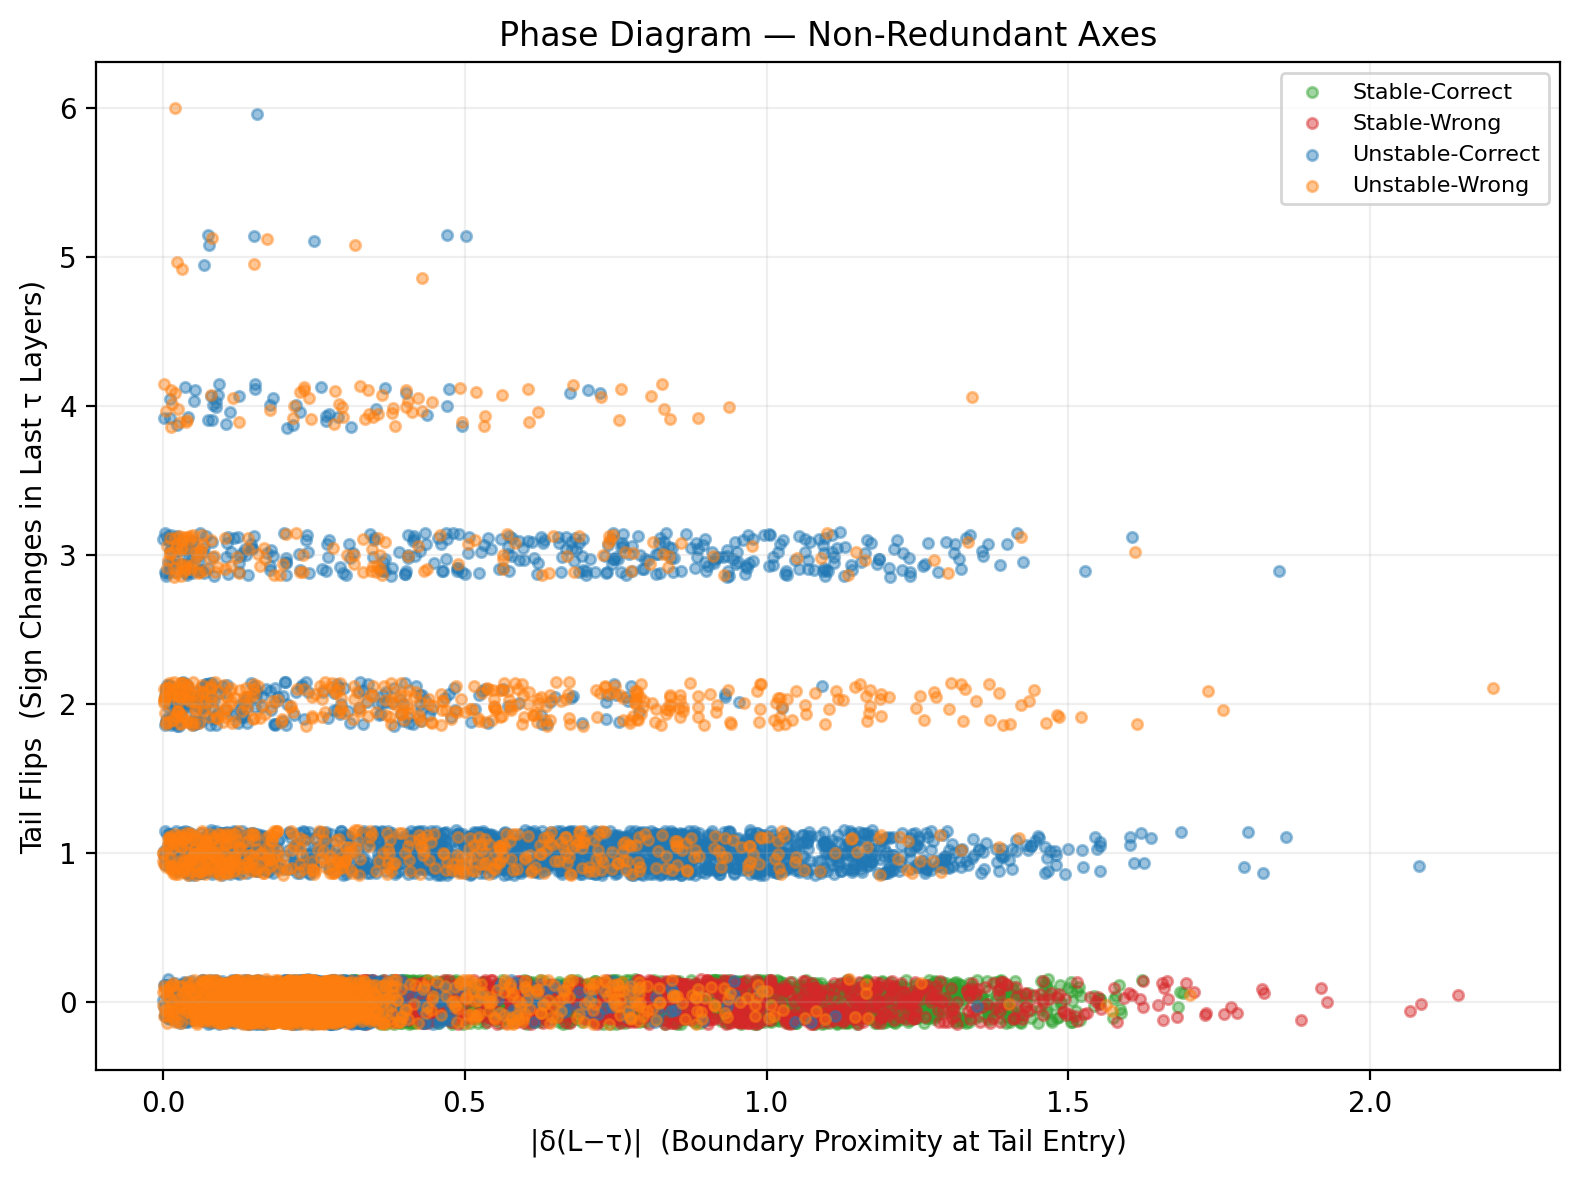
\includegraphics[width=\columnwidth]{fig2_phase_diagram.png}}
    \caption{Phase diagram with non-redundant axes.  $x$-axis: boundary proximity at tail entry $|\delta(L{-}\tau)|$; $y$-axis: number of sign flips in the last $\tau$ layers.  Each point is one prompt~$\times$~model pair.}
    \label{fig:phase}
  \end{center}
\end{figure}


\subsection{Cross-Model and Cross-Domain Replication}

The phase structure replicates qualitatively across all three models.  Absolute magnitudes differ---Qwen produces larger $|\delta|$ than Mistral---but the four-region geometry and the separation between stable and unstable types are consistent.  Domain shifts the \emph{proportion} of types but not the geometry.

\emph{Caveat.}  The clean separation partly reflects our threshold choices.  Clusters remain visually distinct under perturbations ($\tau \in \{6, 8, 10\}$, $b_{\min} \in \{0.1, 0.3, 0.5\}$), but the boundary between stable and unstable is a convention, not a phase transition.


%% ============================================================
%% 5. TWO-FORCE DECOMPOSITION
%% ============================================================
\section{Drift Decomposition}
\label{sec:decomposition}

\subsection{Setup}

At each layer, the residual stream update sums two components: the attention sub-layer output and the MLP sub-layer output.  We extract both at the answer-token position and project each onto a \textbf{decision direction}:
\begin{equation}
  d = e_c - e_{k^*},
  \label{eq:direction}
\end{equation}
where $e_c$ and $e_{k^*}$ are one-hot vectors for the correct and competitor tokens.  The \textbf{attention scalar} $s_{\mathrm{attn}}(l)$ and \textbf{MLP scalar} $s_{\mathrm{mlp}}(l)$ are the dot products of the respective outputs with $d$ after applying the unembedding matrix.

\subsection{Drift Reconstruction}

Observed drift should be approximated by:
\begin{equation}
  g(l) \approx \alpha \cdot s_{\mathrm{attn}}(l) + \beta \cdot s_{\mathrm{mlp}}(l) + \varepsilon.
  \label{eq:decomposition}
\end{equation}
We fit via OLS on a 70/30 train/test split (at the prompt level).  The pipeline requires $R^2 \geq 0.70$ on test data; this gate was pre-registered.

\emph{Why linear?}  A richer model would fit better but explain less.  The residual $\varepsilon$ captures layer-norm effects, cross-term dependencies, and nonlinear interactions.

\subsection{Which Component Drives Which Outcome?}

\cref{fig:decomposition} reveals two key patterns:

\textbf{Attention dominates early steering.}  In layers 0--15, the attention scalar accounts for the majority of positive drift in stable-correct trajectories---consistent with ``routing'' evidence-bearing spans toward the answer position.

\textbf{MLP dominates late commitment.}  In layers 20--28, the MLP scalar grows in magnitude and can drive the final push toward or away from the correct answer.  For stable-wrong trajectories, MLP injection maintains wrong-answer commitment in late layers.

For unstable trajectories, the two components are often \emph{misaligned}: attention pushes one direction while MLP pushes the other, producing oscillatory drift.

\begin{figure}[t]
  \vskip 0.1in
  \begin{center}
    \centerline{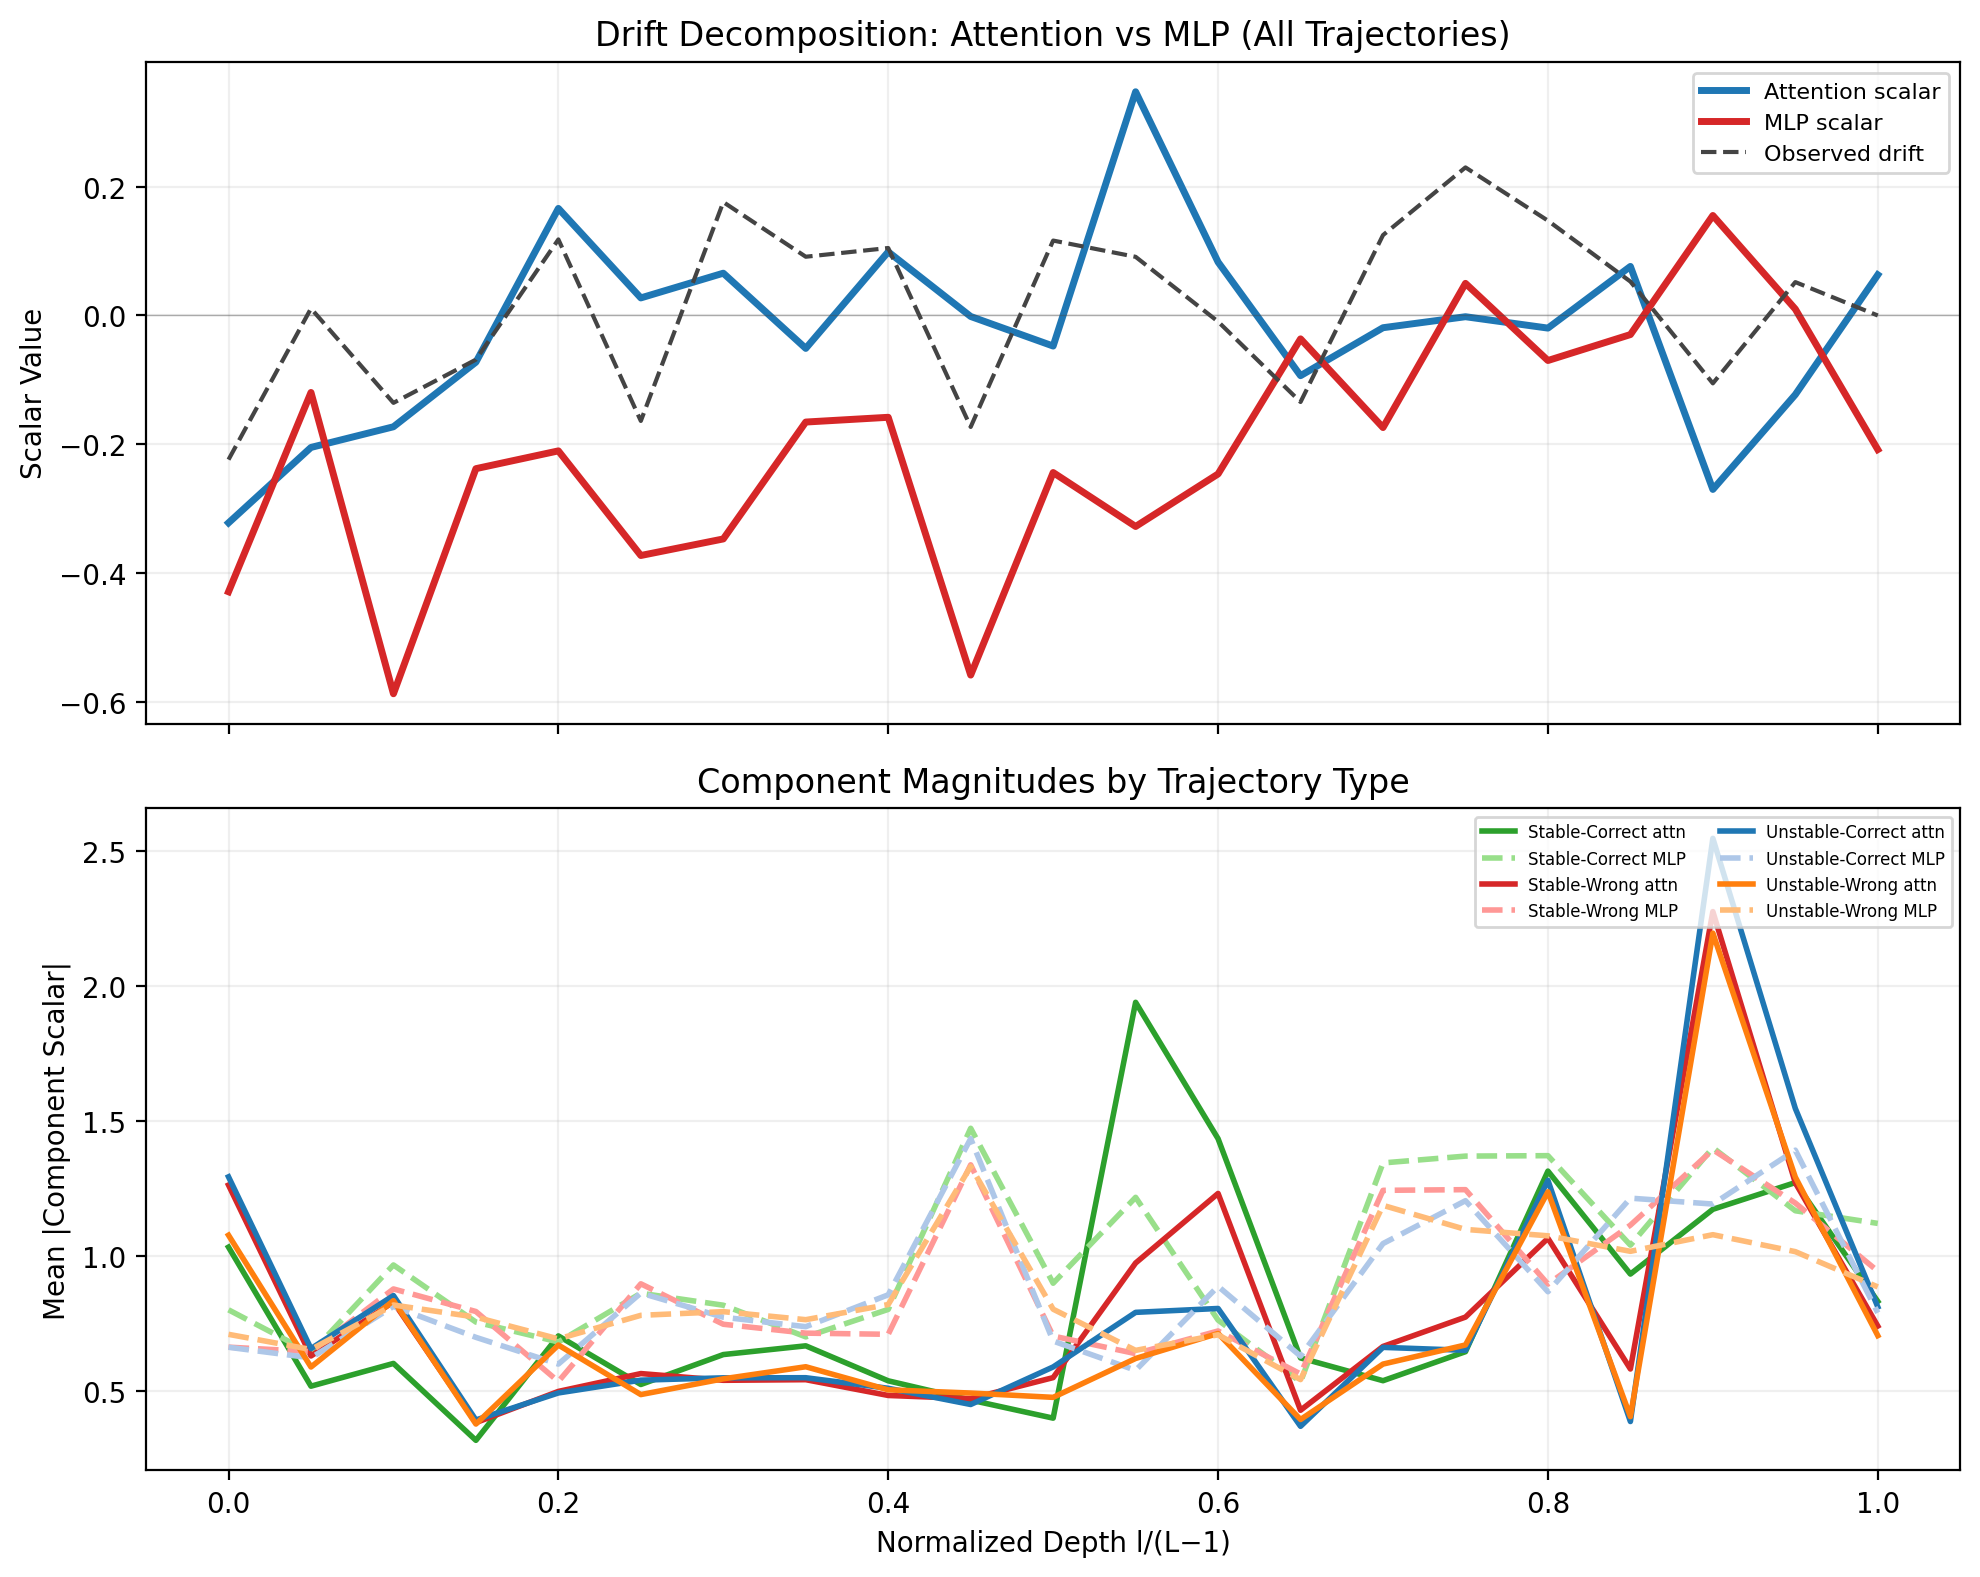
\includegraphics[width=\columnwidth]{fig3_decomposition.png}}
    \caption{\textbf{Top:}~Per-layer drift decomposition into attention and MLP components, with layer depth normalized to $[0,1]$ across models ($R^2 > 0.70$).  \textbf{Bottom:}~Mean absolute component magnitudes by trajectory type.}
    \label{fig:decomposition}
  \end{center}
\end{figure}


%% ============================================================
%% 6. ATTENTION AS ROUTING
%% ============================================================
\section{Attention and Span Routing}
\label{sec:routing}

\subsection{Prompt Span Taxonomy}

Multiple-choice prompts have natural structure: \emph{instruction}, \emph{question stem}, and \emph{option spans} (A--D).  We parse these via regex-based boundary detection.  For analysis, option spans are re-indexed \emph{relative to correctness}: \texttt{option\_correct} (the ground-truth answer), \texttt{option\_competitor} (the strongest wrong option at the final layer), and \texttt{option\_other} (remaining wrong options, averaged).

\subsection{Span Labeling via Counterfactual Effect (Operational Definition)}

We \emph{define} evidence and distractor spans operationally via counterfactual deletion.  For each span $s$, we delete it and re-run inference.  The span effect is $\mathrm{effect}(s) = \delta_{\mathrm{full}} - \delta_{\mathrm{mutated}}$.  Spans with effect $\geq 0.05$ are labeled \emph{evidence}; $\leq -0.05$ are \emph{distractor}; otherwise \emph{neutral}.

\emph{Important:} Because evidence/distractor labels are assigned using the same quantity ($\Delta$) that we later report, the observation that evidence spans have larger $\Delta$ than distractor spans is \emph{true by construction} and does not constitute independent validation of the labels.  We treat this labeling as a useful operational definition rather than a finding.

Label stability under paraphrase requires $\geq 85\%$ agreement and $\geq 0.80$ Jaccard similarity.

\subsection{Attention Mass vs.\ Contribution}

We distinguish \textbf{attention mass} (raw weight from answer position to span tokens, normalized per token) from \textbf{decision-aligned contribution} (the attention output projected onto $d$).

\cref{fig:routing} shows heatmaps with option columns indexed relative to correctness.  Stable-correct trajectories route disproportionate mass per token to \texttt{option\_correct} with large positive contribution.  Stable-wrong trajectories route to \texttt{option\_competitor}.

\begin{figure*}[t]
  \vskip 0.1in
  \begin{center}
    \centerline{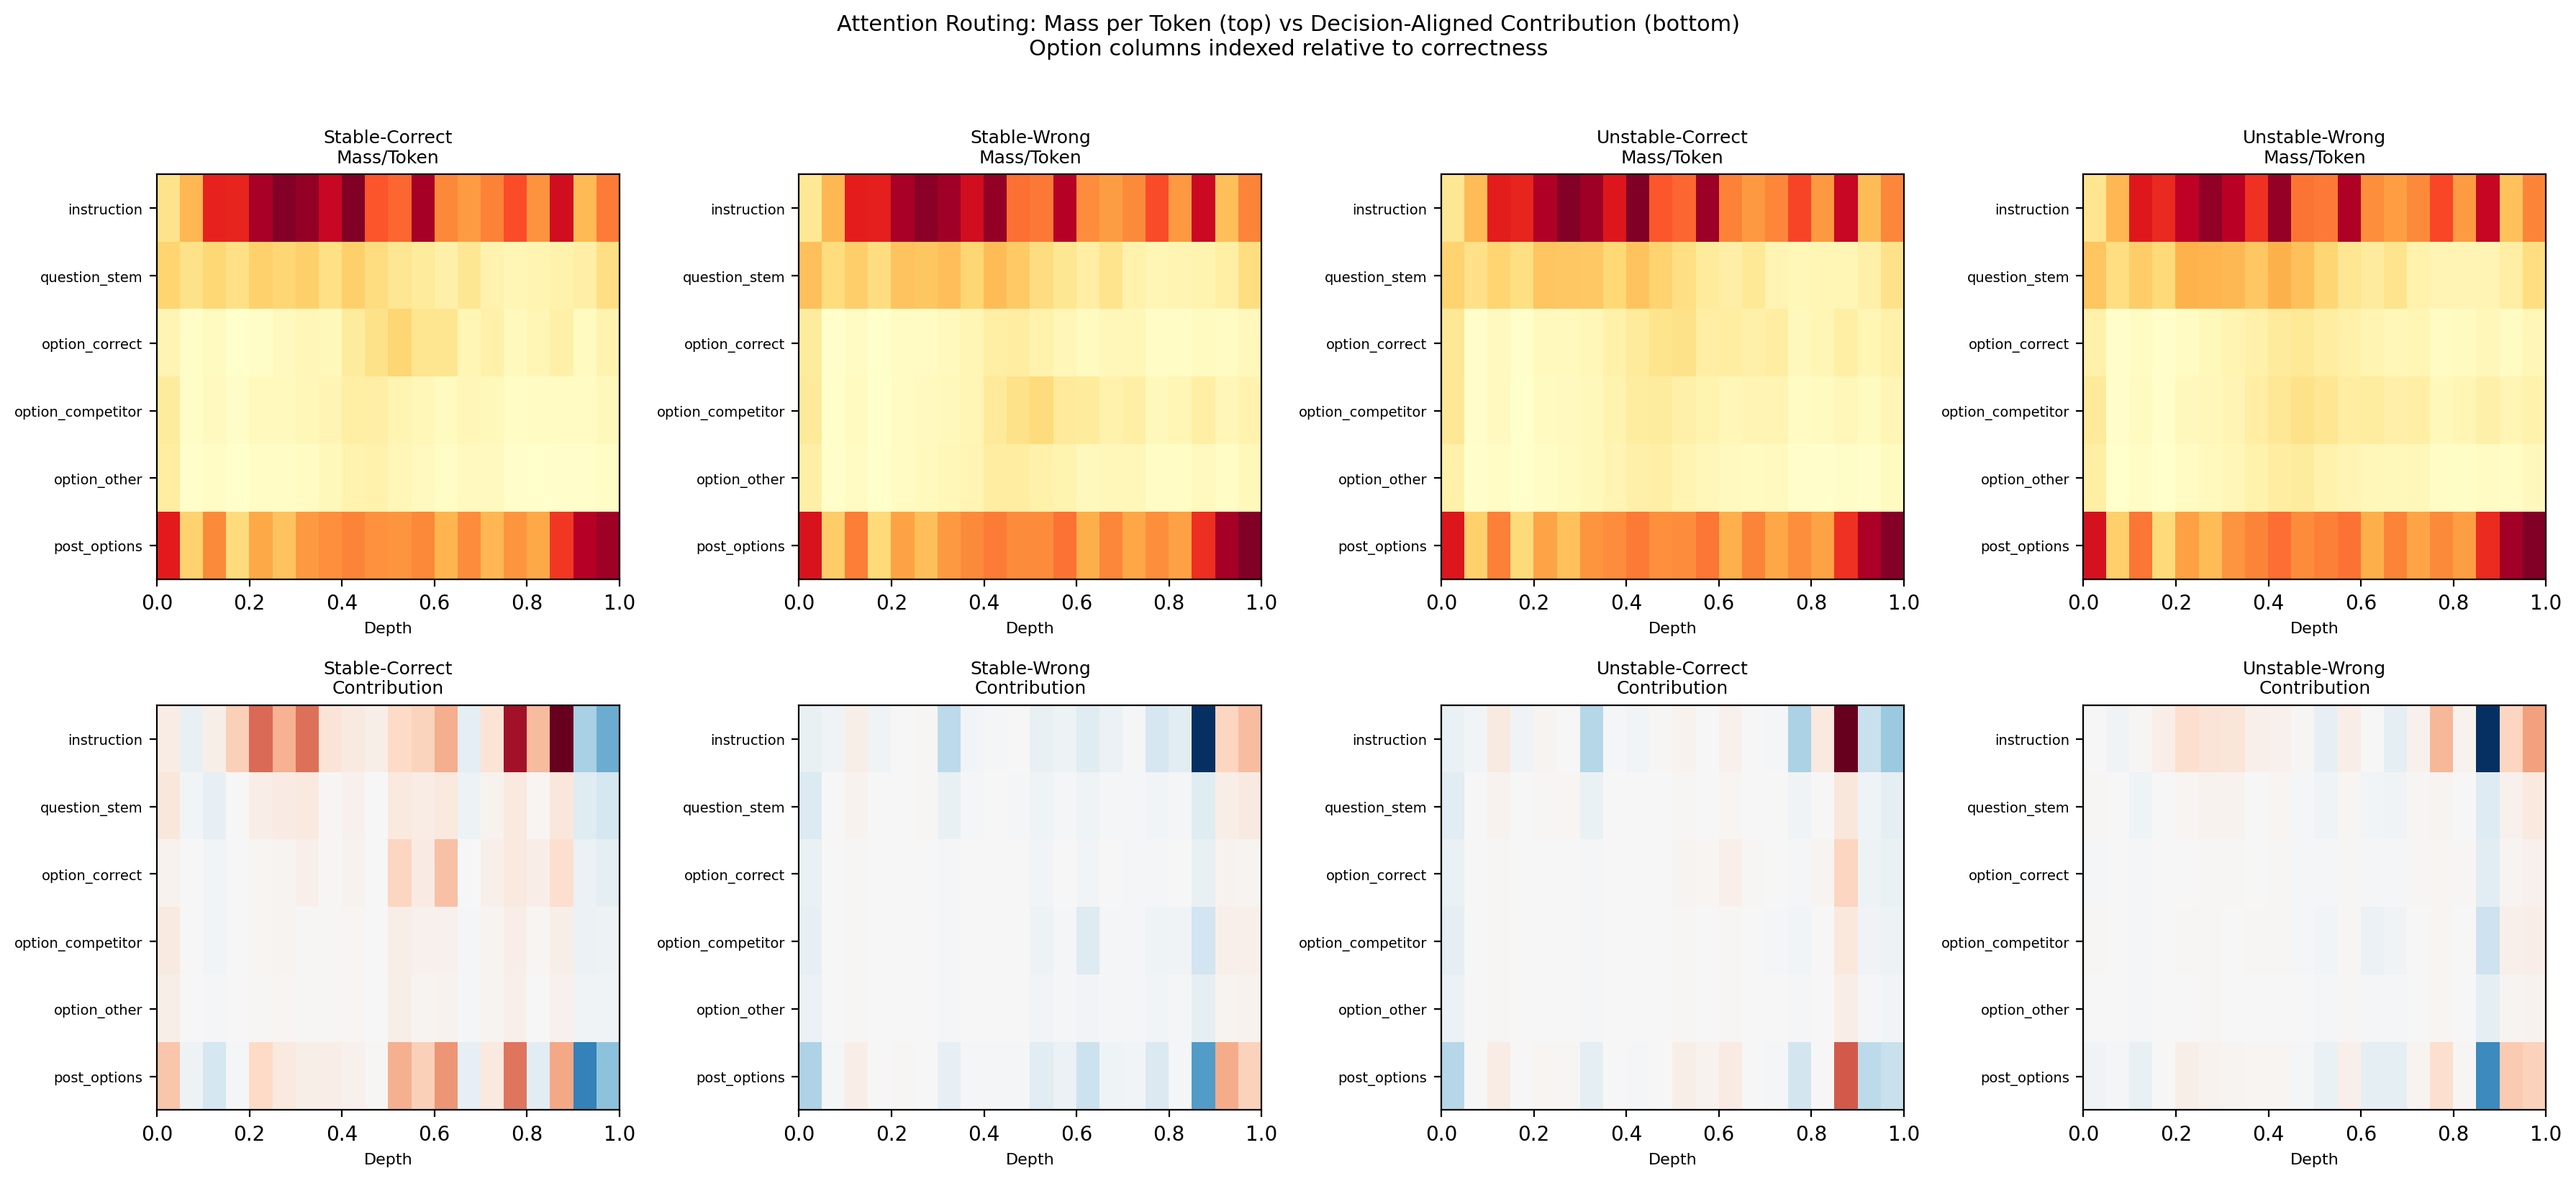
\includegraphics[width=0.95\textwidth]{fig5_attention_routing.png}}
    \caption{Attention routing with option spans indexed relative to correctness.  \textbf{Top row:}~Attention mass per token by trajectory type across normalized depth.  \textbf{Bottom row:}~Decision-aligned contribution.  Columns: \texttt{option\_correct}, \texttt{option\_competitor}, \texttt{option\_other}.}
    \label{fig:routing}
  \end{center}
\end{figure*}


%% ============================================================
%% 7. MLP AS INJECTION
%% ============================================================
\section{MLP Contributions}
\label{sec:mlp}

The MLP scalar $s_{\mathrm{mlp}}(l)$ measures how much parametric knowledge each layer's feedforward network contributes to the decision margin.  Unlike attention, MLP can introduce information absent from the input---stored associations, factual recall, and learned biases.

\textbf{Help regime} (layers 5--20, stable-correct): MLP scalars are moderately positive, reinforcing what attention has routed.

\textbf{Harm regime} (layers 20--28, stable-wrong): MLP scalars are strongly aligned with the wrong answer, actively opposing correct-option routing.  This is pronounced in STEM domains where the MLP appears to inject confidently \emph{wrong} associations.

\textbf{Garbage in, amplified out.}  For unstable-wrong trajectories, attention routes noisy signals in early layers; MLP amplifies this noise in later layers.  Instability is \emph{created}, not merely revealed, by MLP acting on a poorly conditioned routing signal.


%% ============================================================
%% 8. CAUSAL VALIDATION
%% ============================================================
\section{Counterfactual Accounting Experiments}
\label{sec:causal}

Sections~\ref{sec:decomposition}--\ref{sec:mlp} are correlational.  We conduct three families of counterfactual experiments.  The first two (simulated removal and substitution) operate on a \emph{linearized drift-bookkeeping model} rather than full forward-pass interventions; only span deletion involves true input-level interventions with full re-inference.

\subsection{Simulated Component Removal}

We estimate the effect of removing a component by subtracting its scalar from drift at target layers ($l = 20,\ldots,27$) and recomputing the counterfactual final margin:
\begin{equation}
  \delta^{\mathrm{cf}}_L = \delta_0 + \sum_{l=0}^{L-1}\! \left[g(l) - \mathbb{1}[l \in T]\cdot s_{\mathrm{comp}}(l)\right]\!.
  \label{eq:ablation}
\end{equation}
This is a \emph{linearized counterfactual estimate}: it assumes that later layers do not adapt to the modified intermediate state.  Both attention and MLP removal produce finite, directionally consistent shifts across all three models (\cref{fig:causal}a).

\subsection{Simulated Activation Substitution}

We substitute the component scalar from a \emph{successful} trajectory into a \emph{failing} trajectory at target layers, again under the linearized drift model.  Substituting attention scalars from stable-correct into stable-wrong produces positive $\Delta\delta$ for the majority of pairs (\cref{fig:causal}b).  MLP substitution is less consistent, reflecting prompt-specific knowledge.

\subsection{Span Deletion (True Input-Level Intervention)}

Span deletion is the only experiment in this section that involves re-running inference and is therefore a true counterfactual intervention.  \cref{fig:causal}c shows the distribution of $\Delta = \delta_{\mathrm{full}} - \delta_{\mathrm{deleted}}$ by operationally defined span type.  As noted in \cref{sec:routing}, evidence spans have positive $\Delta$ and distractor spans have negative $\Delta$ \emph{by construction}, since these labels are defined by the sign and magnitude of $\Delta$.  The figure displays span-type distributions rather than validation of the labeling.

\subsection{Negative Controls}

Two controls: (1)~\textbf{shuffled}---permuting span labels 256 times; (2)~\textbf{sign-flipped}---randomly flipping effect signs 256 times.  Both baselines center near zero.  The observed evidence-labeled mean exceeds both by $\geq 0.05$.

\paragraph{Limitations of linearized counterfactual accounting.}  Simulated component removal and substitution operate on a drift-bookkeeping model.  They are \emph{not} full forward-pass interventions: later layers are not allowed to react to the modified state.  These estimates are valid under a linearity assumption that has not been independently verified here.  True in-graph ablation and activation patching would provide stronger evidence but would require additional model runs, which are outside the scope of this study.


\begin{figure*}[t]
  \vskip 0.1in
  \begin{center}
    \centerline{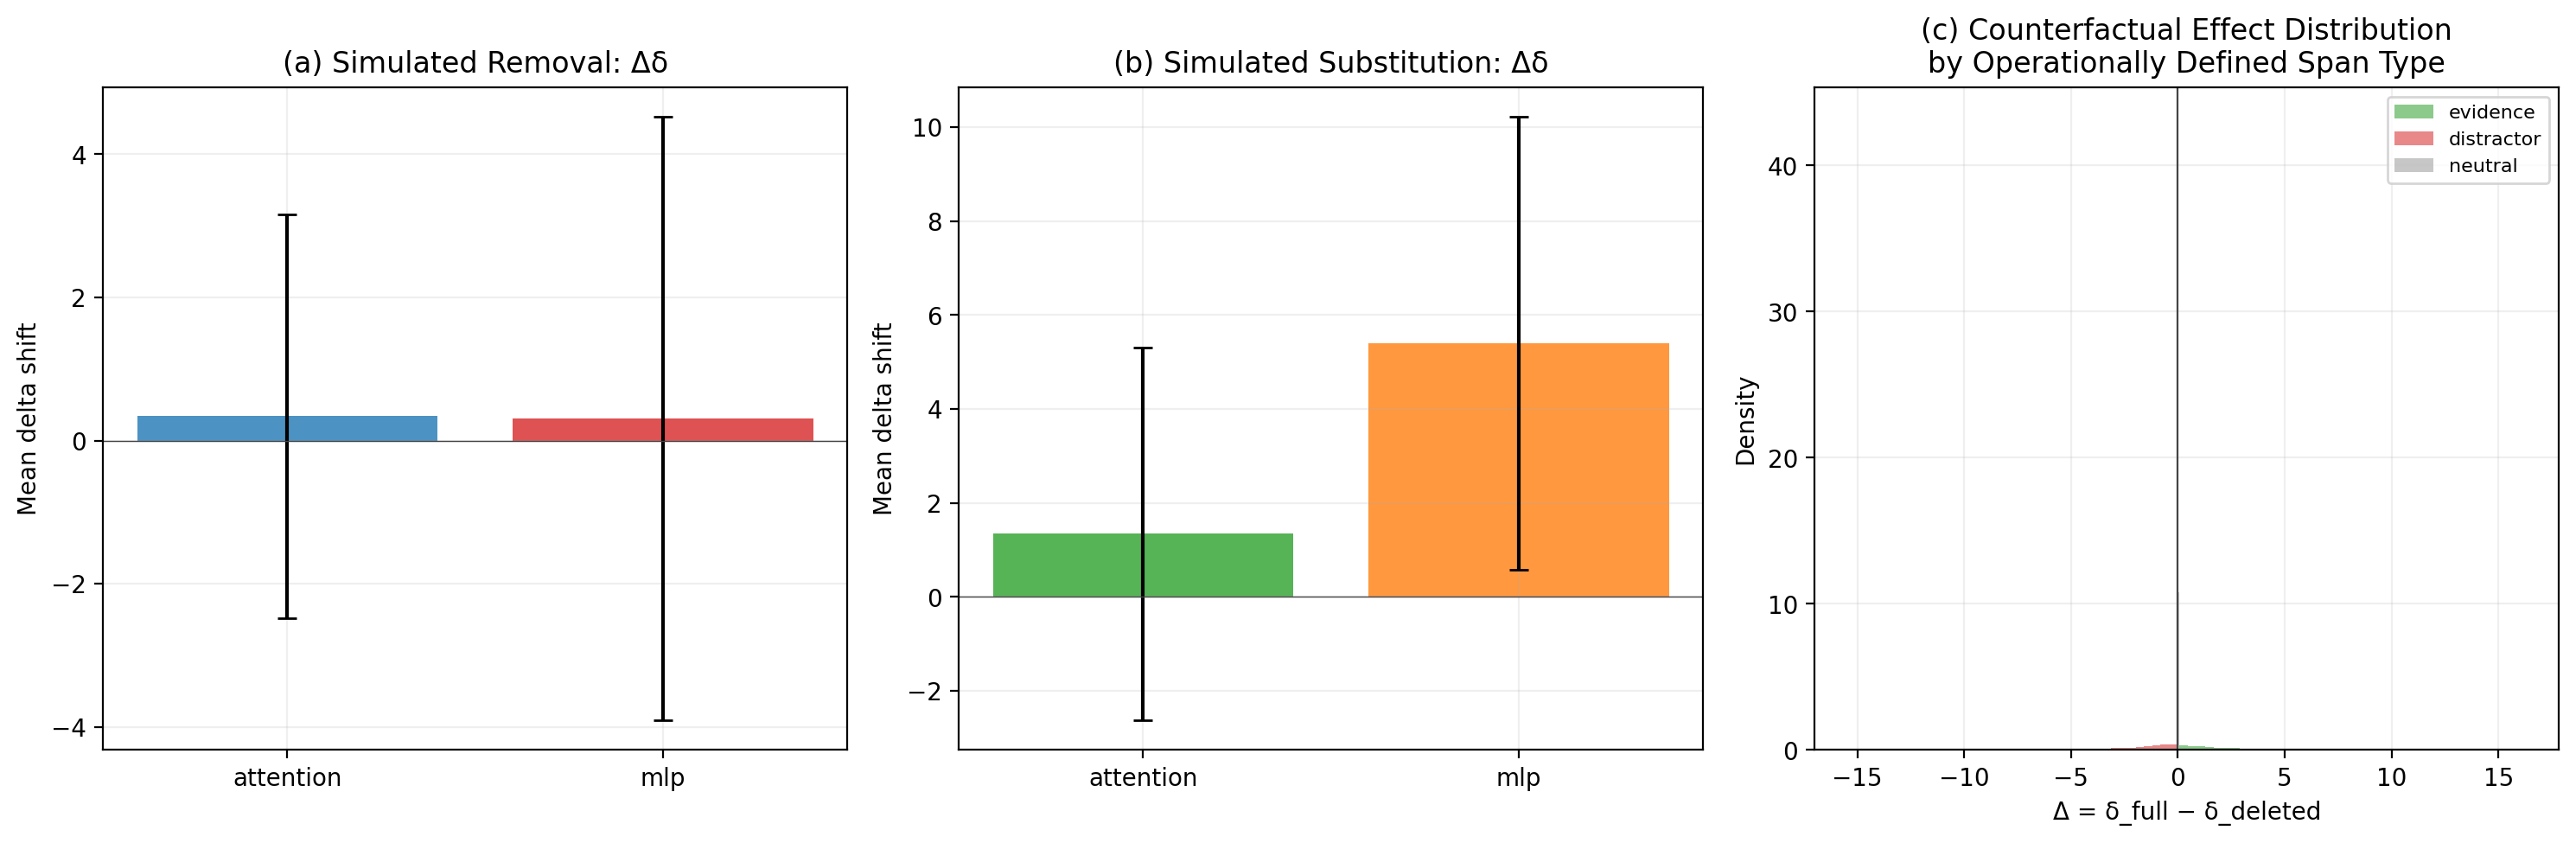
\includegraphics[width=0.95\textwidth]{fig4_causal_validation.png}}
    \caption{Counterfactual accounting.  \textbf{(a)}~Simulated component removal: removing attention from stable-correct decreases $\delta$; removing MLP from stable-wrong increases $\delta$.  \textbf{(b)}~Simulated activation substitution shifts failing trajectories positive.  \textbf{(c)}~Distribution of counterfactual effect $\Delta$ by operationally defined span type.  Evidence/distractor separation is by construction (see \S\ref{sec:routing}).}
    \label{fig:causal}
  \end{center}
\end{figure*}



%% ============================================================
%% 9. DISCUSSION
%% ============================================================
\section{Discussion}
\label{sec:discussion}

\paragraph{Code.}  Repository: \url{https://github.com/gut-puncture/The-Shape-of-Wisdom}.

\textbf{What the primitives buy.}  Rather than ``the model got it wrong,'' we can say ``the model entered the correct region at layer~12 but was pushed out by MLP injection at layer~23.''  This localizes failure, identifies the responsible component, and suggests targeted interventions.

\textbf{Implications for training.}  We refrain from strong claims but note a hypothesis: training procedures that penalize drift disagreement between attention and MLP in late layers might reduce stable-wrong rates.

\textbf{Limitations.}
\vspace{-0.5em}
\begin{enumerate}\setlength{\itemsep}{0pt}
\item \textbf{Restricted-choice readout.}  All quantities live in a 4-token logit subspace (\{A,B,C,D\}); full hidden-state and vocabulary structure may be missed.
\item \textbf{Linear decomposition.}  Up to 30\% of variance remains in $\varepsilon$.
\item \textbf{Linearized counterfactual accounting.}  Component removal and substitution experiments use a drift-bookkeeping model, not full forward-pass interventions.  Later layers are not allowed to react to modified states.
\item \textbf{Circular span labeling.}  Evidence/distractor labels are defined by counterfactual effect on $\delta$, so their separation by $\Delta$ is tautological rather than a finding (see \S\ref{sec:routing}).
\item \textbf{Scale.}  Only 7--8B models studied.
\item \textbf{Prompt format.}  Only four-choice MC; open-ended generation may differ.
\item \textbf{Threshold sensitivity.}  Classification depends on pre-registered but conventional thresholds.
\item \textbf{Single run.}  Results from one deterministic run (seed 12345).
\end{enumerate}


%% ============================================================
%% 10. RELATED WORK
%% ============================================================
\section{Related Work}

\textbf{Logit lens and tuned lens.}  \citet{nostalgebraist2020} and \citet{belrose2023} project intermediate representations through the unembedding matrix.  We analyze the \emph{trajectory} of projections across layers in the answer-token subspace.

\textbf{Mechanistic interpretability.}  The circuits paradigm~\cite{elhage2021,olsson2022,conmy2023} identifies computational subgraphs.  We characterize trajectory-level dynamics, trading microscopic precision for macroscopic coverage.

\textbf{Probing classifiers.}  Linear probes~\cite{belinkov2022,hewitt2019} test whether representations encode specific properties.  Our $\delta(l)$ is a targeted probe without learned-classifier ambiguity.

\textbf{Causal tracing.}  \citet{meng2022} localize factual associations.  Our span-deletion tests operate at the prompt level; ablations target component types rather than individual positions.

\textbf{Decision dynamics.}  Recent work~\cite{din2023,geva2023} studies layerwise prediction evolution.  We contribute a unified framework connecting descriptive dynamics, mechanistic decomposition, and counterfactual accounting.


%% ============================================================
%% 11. CONCLUSION
%% ============================================================
\section{Conclusion}

A transformer's decision on a multiple-choice question is not a point but a trajectory.  Three measurable quantities---the logit margin $\delta$, its per-layer drift $g$, and the boundary distance $|\delta|$---suffice to classify this trajectory into four outcome types, producing a phase diagram that replicates across architectures and domains.  Decomposing drift into attention routing and MLP injection reveals that attention steers early, MLP commits late, and their disagreement creates instability.  Counterfactual accounting experiments---both linearized estimates and true input-level span deletions---confirm directionally consistent effects.

The framework is deliberately modest: we claim sufficiency for classification, not necessity; counterfactual relevance under linearity assumptions, not sole causation; and insight from a restricted-choice logit-margin space, not complete representation coverage.  The phase diagram is a map.  The two-force decomposition is a compass.  Together, they provide a vocabulary for navigating the space between a prompt and an answer.


\begin{figure*}[t]
  \vskip 0.1in
  \begin{center}
    \centerline{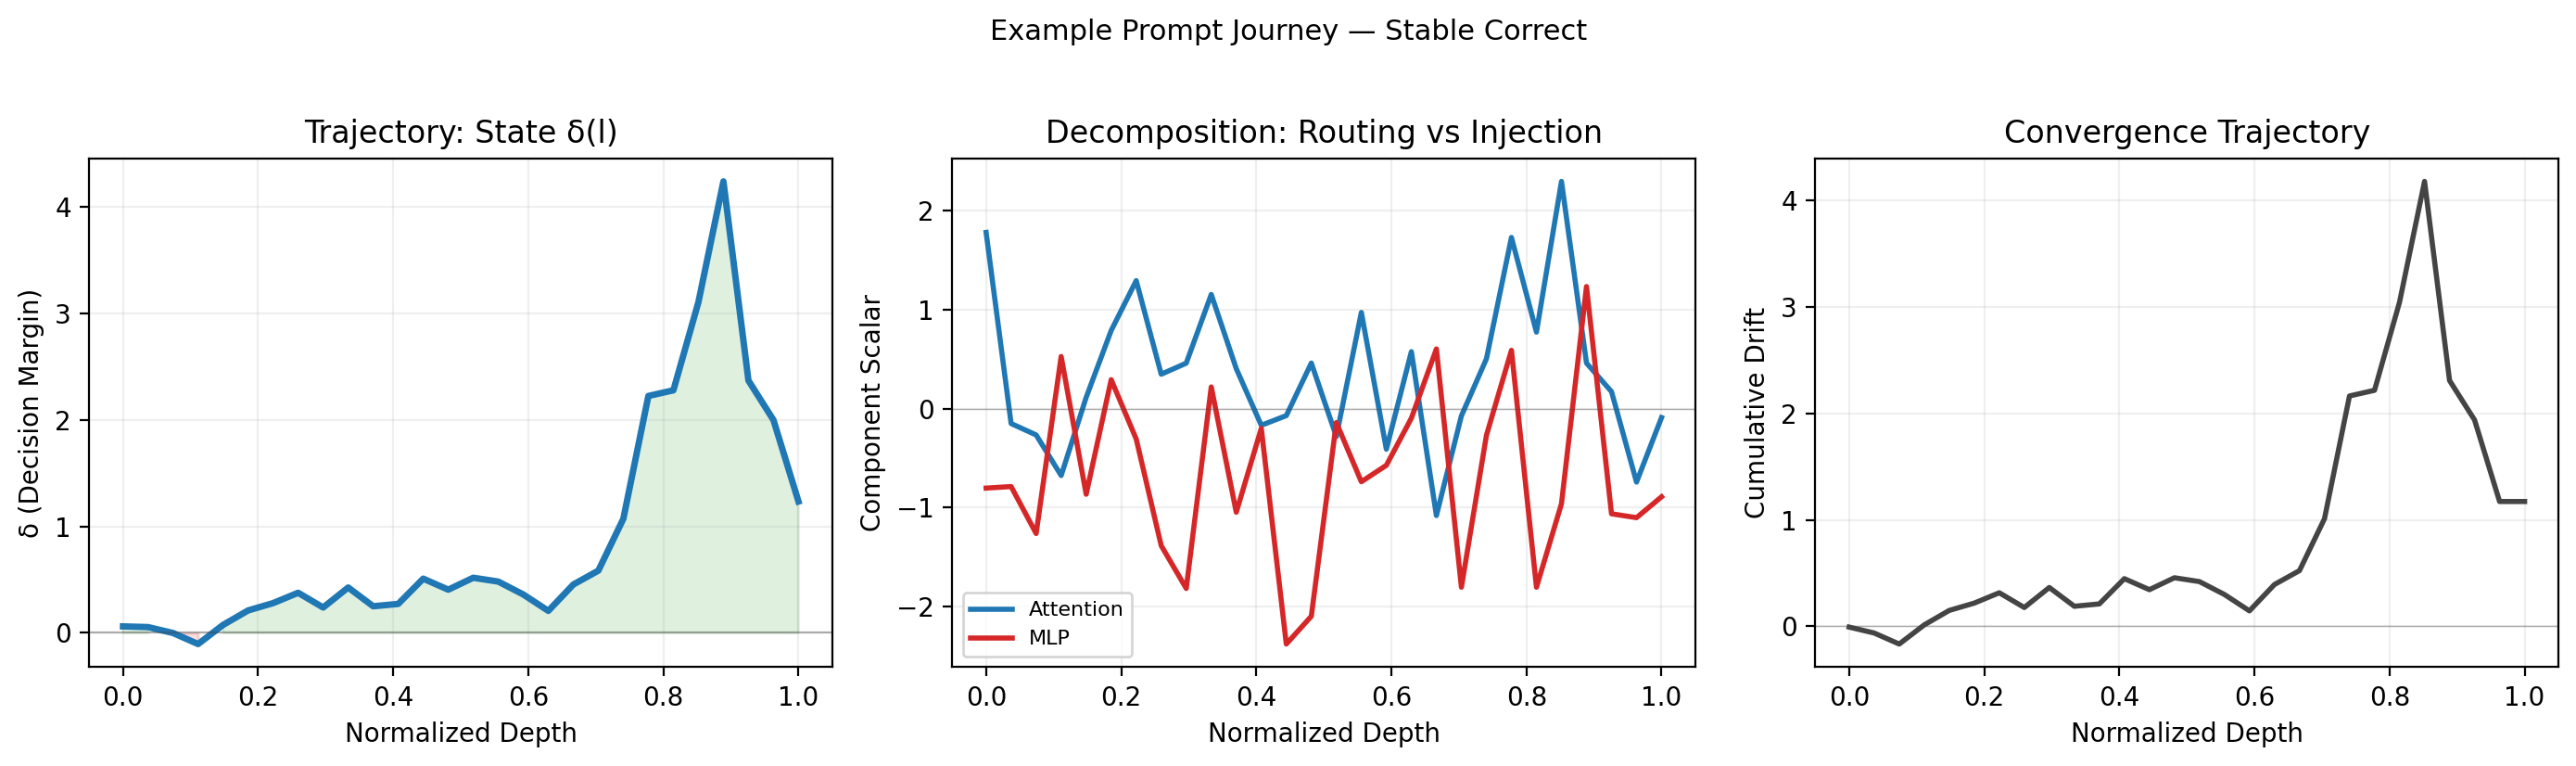
\includegraphics[width=0.90\textwidth]{fig6_prompt_flow.png}}
    \caption{A prompt's journey through decision space with normalized depth axis.  \textbf{Left:}~Decision margin $\delta$ trajectory.  \textbf{Center:}~Attention and MLP scalar decomposition.  \textbf{Right:}~Cumulative drift convergence.}
    \label{fig:flow}
  \end{center}
\end{figure*}


%% ============================================================
%% IMPACT STATEMENT
%% ============================================================
\section*{Impact Statement}

This paper presents work whose goal is to advance the field of mechanistic interpretability by providing diagnostic tools for understanding transformer decision-making.  Improved understanding of model failures may contribute to safer and more reliable AI systems.  We do not foresee specific negative societal consequences beyond those generally associated with advances in machine learning.


%% ============================================================
%% REFERENCES
%% ============================================================
\balance
\bibliography{references}
\bibliographystyle{plainnat}


%% ============================================================
%% APPENDIX
%% ============================================================
\clearpage
\appendix

\section{Threshold Sensitivity Analysis}
\label{sec:appendix_sensitivity}

We vary the trajectory classification parameters and verify that the four-cluster structure persists.

\textbf{Tail length $\tau \in \{6, 8, 10\}$:}  Shorter tails classify more trajectories as stable; longer tails classify more as unstable.  Phase geometry is preserved.

\textbf{Minimum boundary $b_{\min} \in \{0.1, 0.3, 0.5\}$:}  Lower thresholds admit near-boundary trajectories as stable; higher thresholds reclassify them.  Separation degrades gracefully.

\textbf{Late flip threshold $\in \{0, 1\}$:}  Allowing one flip expands the stable class modestly for $\tau = 8$.

\section{Probability-Space Comparison}
\label{sec:appendix_prob}

Replicating the phase diagram using probability margins ($p_c - p_{k^*}$) in place of logit margins produces visible but less separated clusters.  High-confidence decisions compress into a narrow probability range, reducing discrimination.  We recommend logit-space analysis for trajectory work.

\section{PCA Visualizations of Hidden States}
\label{sec:appendix_pca}

PCA on full hidden-state vectors at selected layers shows partially separable trajectory-type clusters in PC1--PC2 space.  However, explained variance is below 15\% for PC1, making these visualizations illustrative rather than evidentiary.

\section{Decomposition Residual Analysis}

The residual $\varepsilon$ from \cref{eq:decomposition} has mean near zero with modest layer-dependent heteroscedasticity (larger variance at layers 12--18).  No systematic bias invalidates the linear approximation.

\section{Per-Domain Breakdowns}

STEM domains show higher stable-wrong rates (confident factual errors).  Humanities show higher instability (ambiguous or context-dependent questions).  Social sciences are intermediate.

\section{Methods}
\label{sec:methods}

\textbf{Metric computation.}  For each prompt~$\times$~model pair, layerwise candidate logits for the four answer tokens (A/B/C/D) are extracted from every transformer block.  All logits and probabilities are computed over this \emph{restricted four-candidate subspace} only; correctness is argmax within $\{\mathrm{A},\mathrm{B},\mathrm{C},\mathrm{D}\}$ at the final layer.  $\delta(l)$, $g(l)$, $b(l)$, and $k^*(l)$ are computed per \cref{sec:primitives}.  Probabilities are softmax-normalized over four candidates; entropy is $H(l) = -\!\sum_c p_c(l)\log p_c(l)$ with clipping at $10^{-12}$.

\textbf{Layer indexing.}  Models in this study have different layer counts (Qwen: 28, Llama: 32, Mistral: 32).  Cross-model figures use \emph{normalized depth} $l/(L{-}1) \in [0,1]$ to enable comparison.

\textbf{Trajectory classification.}  Sign flips are computed on the sign sequence of $\delta$, ignoring zeros.  Late flips are restricted to the tail window.  Stability requires zero late flips and $\min_{l\, \in\, \mathrm{tail}} b(l) \geq 0.3$.

\textbf{Span parsing.}  Prompt spans are identified via regular-expression boundary detection.  Option spans are re-indexed relative to correctness (\texttt{option\_correct}, \texttt{option\_competitor}, \texttt{option\_other}).  Span effects are computed by deletion and re-inference (true input-level intervention).  Evidence/distractor labels are an \emph{operational definition} using symmetric thresholds at $\pm 0.05$; they are not independently validated.  Paraphrase stability is assessed on 50 prompts per model.

\textbf{Tracing and decomposition.}  For the tracing subset, attention and MLP outputs are captured via forward hooks using eager attention.  The decision direction $d$ is computed per \cref{eq:direction}.  OLS fit uses a 70/30 train/test split at the prompt level with $R^2 \geq 0.70$ enforced.

\textbf{Counterfactual experiments.}  Simulated component removal subtracts component scalars at layers 20--27 per \cref{eq:ablation}; this is a linearized estimate, not a forward-pass intervention.  Simulated substitution replaces the failing trajectory's component scalar with the successful trajectory's.  Span deletion actually removes spans and re-runs inference.  Negative controls: label-shuffle (256 permutations) and sign-flip (256 iterations).

\textbf{Statistics.}  Bootstrap CIs use 2{,}000 resamples.  Permutation tests use 5{,}000 permutations.  Multiple-comparison correction uses Benjamini--Hochberg with $\alpha = 0.05$.  All random operations use deterministic seeds.

\textbf{Reproducibility.}  The full pipeline runs from a single orchestrator with fail-closed gating.  Intermediate artifacts are persisted as Parquet files with SHA-256 manifests.  Thermal management enforces checkpoint/resume determinism.

\end{document}
